
% Chapter 4: Results and Analysis

This chapter presents the empirical evaluation of the pipeline that was described in Chapter \ref{chap:methodology} when applied to the LLaMA 3.2 1B Instruct model. The experiments reveal systematic patterns in how different optimization techniques affect performance across multiple evaluation metrics.

Subsequent sections examine compression efficiency, quality degradation, and the interaction effects between sequential optimization stages. Results demonstrate that certain technique combinations achieve substantial parameter reduction while maintaining acceptable capability levels, whereas others exhibit rapid degradation beyond critical compression ratios.

The tables presented in this chapter display a representative subset of the experimental data to highlight key findings and trends. The complete results from all configurations that were tested are available in Appendix \ref{app:appendix1}, along with examples of text generated by selected models.

\section{Pruning Analysis}

The initial phase of experimentation examined the isolated effects of pruning techniques without quantization or recovery mechanisms. A total of 42 pruning-only configurations were evaluated, including 29 combined ones that applied both depth and width pruning simultaneously to assess the compounding effects of multi-dimensional compression.

Table \ref{tab:depth_pruning_results} shows the results from a subset of the complete experimental data, with size measurements reflecting GPU VRAM occupancy on our testing cluster (4x GTX 1080 Ti). Width-pruned variants show no memory reduction despite significant parameter reduction because the inference framework does not exploit structured sparsity patterns for memory optimization, requiring full dense tensor allocation regardless of zero weights. Implementing hardware-accelerated structured sparsity support would address this limitation and is discussed in Section \ref{sec:future_work_engineering}.

{\begin{table}[!htbp]
\centering
\footnotesize
\caption[Results for Pruning-Only Configurations (Subset)]{Results for models which have undergone pruning without quantization or performance recovery. This table presents a subset of results from the complete dataset available in Appendix \ref{app:appendix1}.} \label{tab:pruning_only_results}
\label{tab:depth_pruning_results}
\begin{tabular}{lcccccc}
\hline
\textbf{Config} & \multicolumn{2}{c}{\textbf{TriviaQA (\%) $\uparrow$}} & & \textbf{WikiText $\downarrow$} & \textbf{\#Params} & \textbf{Size} \\
\cline{2-3}
& \textbf{Closed} & \textbf{Open} & & \textbf{PPL} & & \textbf{(GB)} \\
\hline
\textit{Baseline Instruct} & \textit{50.6} & \textit{81.8} & & \textit{26.61} & \textit{1235.8M} & \textit{2.30} \\
Depth 2 & 20.0 & 53.0 & & 55.24 & 1114.2M & 2.08 \\
Depth 4 & 5.6 & 14.2 & & 230.77 & 992.5M & 1.85 \\
Depth 6 & 2.0 & 2.4 & & 2081.04 & 870.9M & 1.62 \\
Depth 8 & 1.2 & 1.4 & & 227734.90 & 749.2M & 1.40 \\
Width 1:2 & 1.8 & 2.2 & & 471.66 & 749.3M & 2.30 \\
Width 2:4 & 7.0 & 17.2 & & 161.10 & 749.3M & 2.30 \\
Width 1:8 & 47.8 & 80.8 & & 27.19 & 1114.2M & 2.30 \\
Width 4:8 & 12.6 & 42.4 & & 81.32 & 749.3M & 2.30 \\
\textbf{Width 1:16} & \textbf{49.2} & \textbf{81.8} & & \textbf{26.77} & \textbf{1175.0M} & \textbf{2.30} \\
Width 8:16 & 16.2 & 52.8 & & 64.08 & 749.3M & 2.30 \\
Width 12:16 & 0.2 & 0.2 & & 1793.97 & 506.0M & 2.30 \\
Depth 2 + Width 1:2 & 0.4 & 0.4 & & 694.34 & 688.4M & 2.08 \\
Depth 2 + Width 2:4 & 3.8 & 5.0 & & 309.32 & 688.4M & 2.08 \\
Depth 2 + Width 1:8 & 20.2 & 53.6 & & 57.22 & 1007.7M & 2.08 \\
Depth 2 + Width 4:8 & 6.4 & 15.2 & & 185.43 & 688.4M & 2.08 \\
Depth 2 + Width 1:16 & 19.6 & 51.6 & & 55.68 & 1061.0M & 2.08 \\
Depth 2 + Width 8:16 & 7.6 & 23.4 & & 139.97 & 688.4M & 2.08 \\
Depth 4 + Width 1:8 & 5.2 & 14.8 & & 244.69 & 901.3M & 1.85 \\
Depth 4 + Width 4:8 & 3.0 & 2.6 & & 774.60 & 627.6M & 1.85 \\
Depth 4 + Width 1:16 & 4.6 & 14.6 & & 235.32 & 946.9M & 1.85 \\
Depth 4 + Width 8:16 & 2.6 & 6.2 & & 591.59 & 627.6M & 1.85 \\
Depth 6 + Width 1:8 & 2.0 & 1.6 & & 2376.63 & 794.9M & 1.62 \\
Depth 6 + Width 4:8 & 0.8 & 1.0 & & 77482.90 & 566.8M & 1.62 \\
Depth 6 + Width 1:16 & 1.8 & 1.6 & & 2032.84 & 832.9M & 1.62 \\
Depth 8 + Width 4:8 & 0.8 & 0.4 & & 554910.71 & 506.0M & 1.40 \\
Depth 8 + Width 3:4 & 0.4 & 0.4 & & 1044840.71 & 384.3M & 1.40 \\

\hline
\end{tabular}
\end{table}
}



\begin{figure}[!htbp]
    \centering
    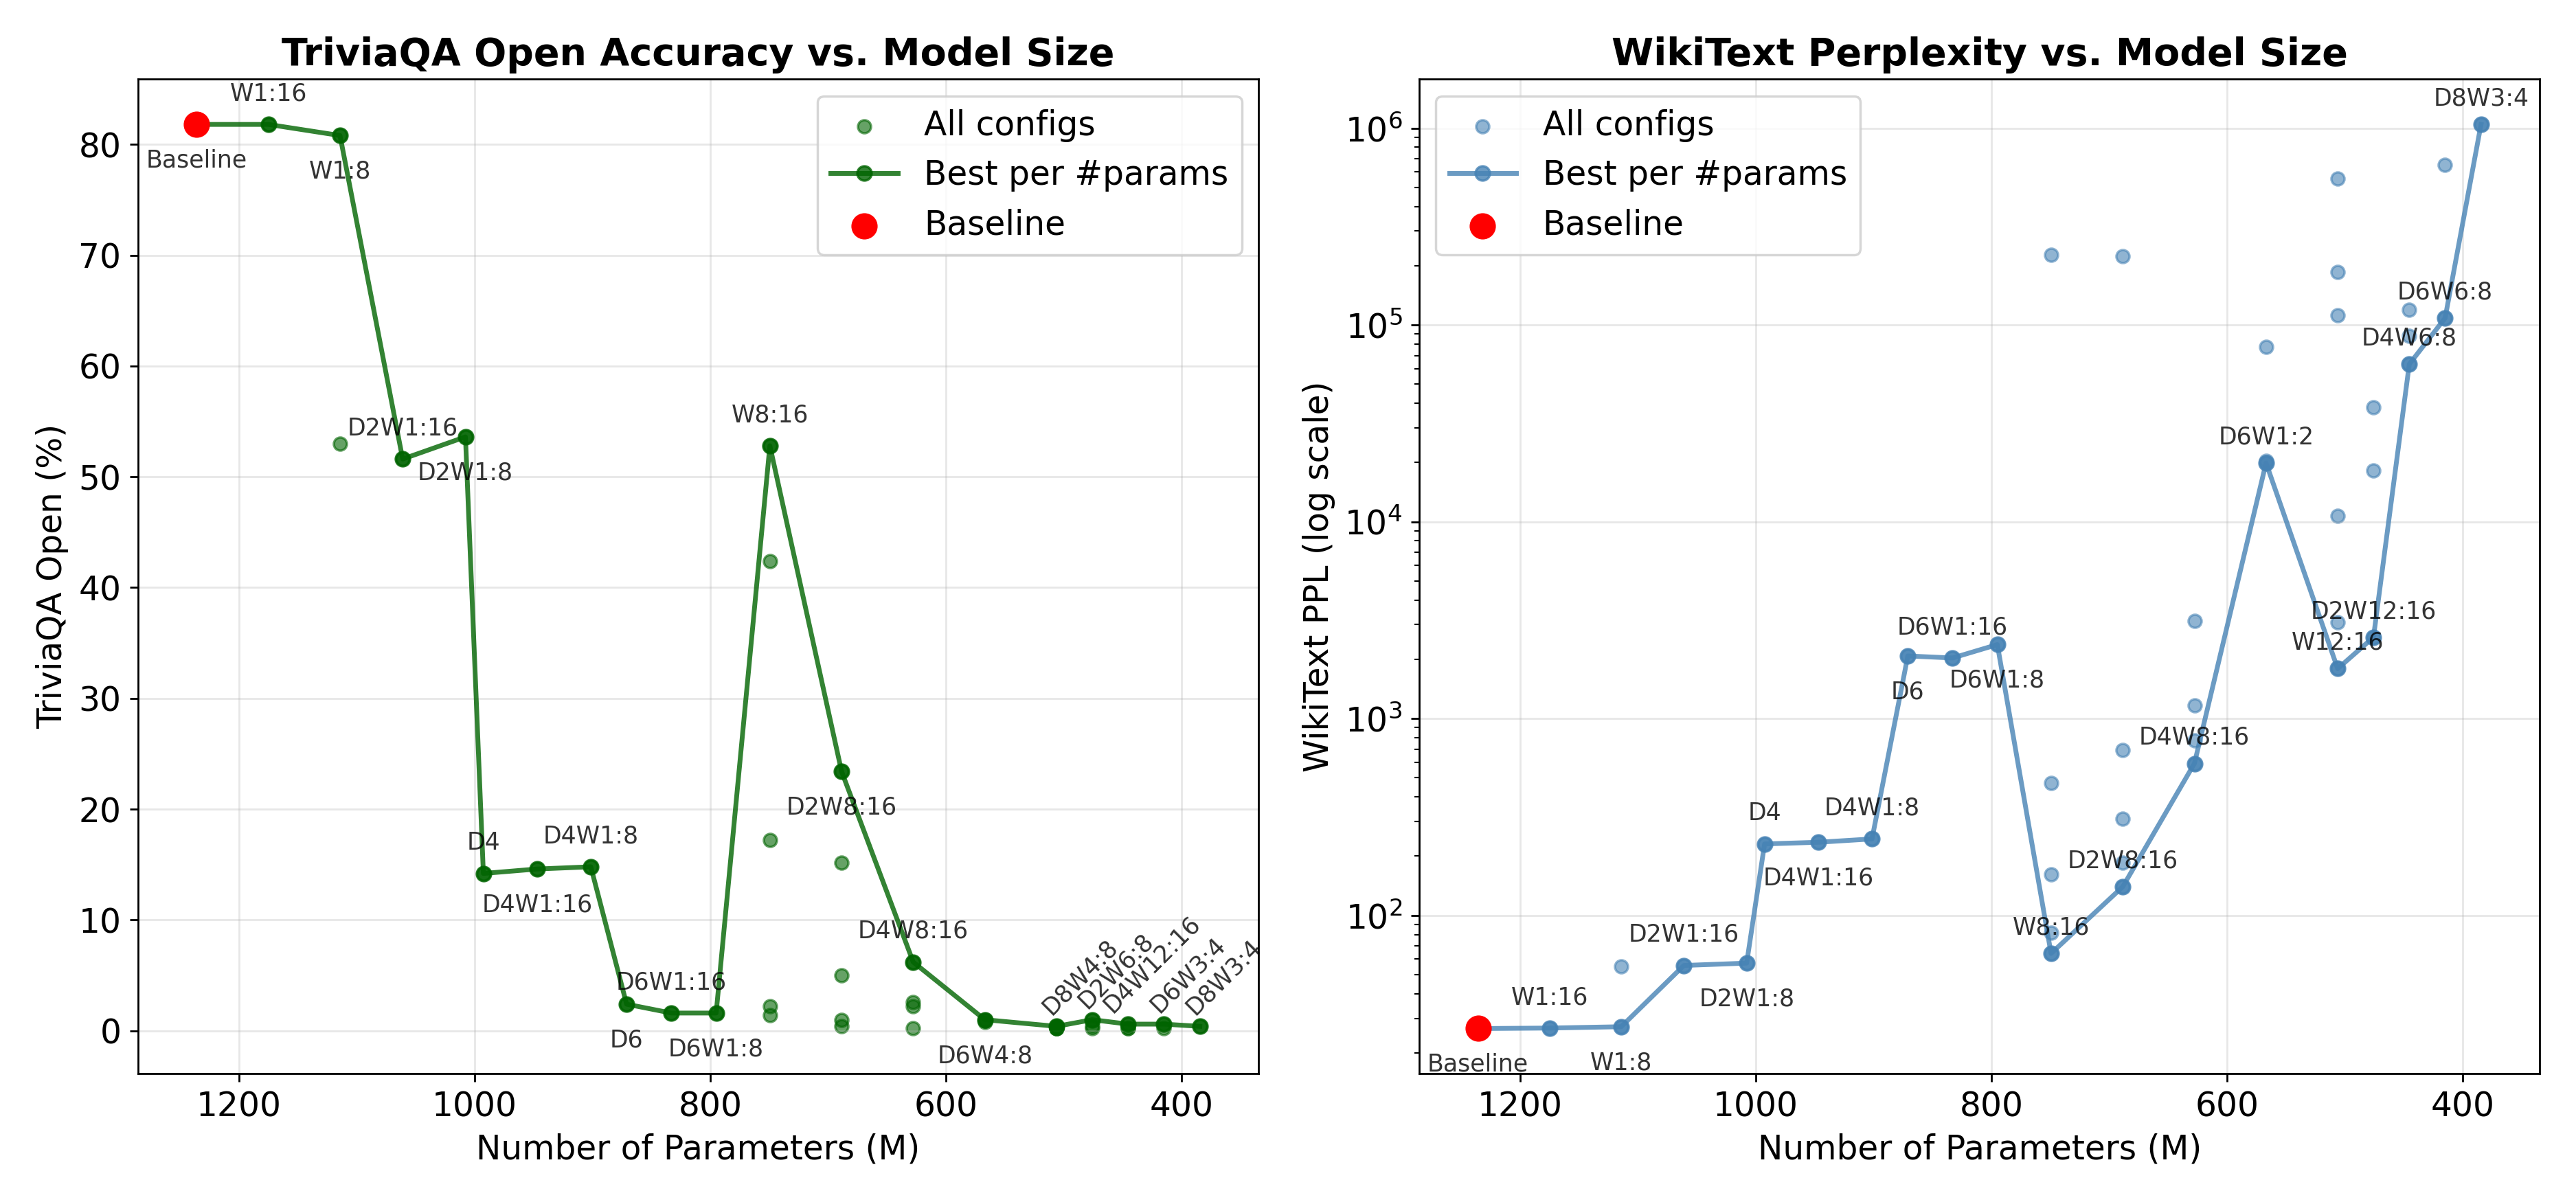
\includegraphics[width=\textwidth]{model_size4.png}
    \caption[Comparison of Pruned Models]{The graph compares performance across parameter counts for models that were pruned without any additional transformations, using TriviaQA Open accuracy and WikiText perplexity as evaluation metrics. The darker line represents the Pareto front, highlighting which pruned models deliver the best results for their given parameter budget without being dominated by smaller, more efficient alternatives.}
    \label{fig:graph_size}
\end{figure}

As evidenced by Figure \ref{fig:graph_size}, the results demonstrate a steep degradation curve where even modest layer removal causes substantial quality deterioration. The most striking observation is the precipitous decline beyond removing two layers. While Depth 2, the variant with 2 layers removed, maintains reasonable functionality with 53.0\% accuracy on TriviaQA's open-book benchmark (i.e. TriviaQA Open) compared to the baseline's 81.8\%, removing four layers causes performance to collapse to just 14.2\%. This suggests that architectural depth in transformer models exhibits critical thresholds beyond which fundamental language capabilities deteriorate rapidly.

The perplexity measurements on WikiText-2 reinforce this pattern, with Depth 2 showing a manageable increase to 55.24 compared to the baseline's 26.61, while deeper pruning leads to catastrophic degradation. Removing eight layers (Depth 8 configuration) causes perplexity to exceed beyond 200,000, indicating near-complete loss of coherent language modeling capability.

On the other hand, width pruning shows markedly different characteristics. The Width 1:8 variant emerges as particularly noteworthy, maintaining 80.8\% accuracy on TriviaQA Open while reducing parameters from 1235.8M to 1114.2M. This represents only a minimal performance drop of 1.0 percentage point while achieving a 10\% reduction in model size, with parameter count comparable to the Depth 2 configuration. The perplexity increase is equally modest, rising from 26.61 to 27.19. This finding suggests that transformer architectures contain significant redundancy in their width dimension when weights are removed judiciously, with the WANDA algorithm's ability to identify and remove less critical weights while preserving essential model capacity proving effective for moderate compression ratios.

However, more aggressive width pruning follows the same catastrophic degradation pattern observed when extensively removing entire layers. The Width 1:2 configuration reduces TriviaQA Open accuracy to just 2.2\%, thus proving that there are clear limits to how extensively models can be compressed through width reduction alone.
Moreover, the granularity of width pruning significantly influences these results, as evidenced by the progression from Width 1:2 (2.2\% TriviaQA Open) to Width 2:4 (17.2\%) to Width 4:8 (42.4\%), showing how different sparsity patterns at the same compression ratio yield vastly different outcomes.

Ultimately, performance of models with combined configurations, without recovery mechanisms, proves unacceptable for practical deployment unless weight removal remains minimal. The only viable exception is Depth 2 + Width 1:8, which maintains 53.6\% accuracy on TriviaQA Open while achieving an 18\% parameter reduction, representing the practical threshold for structural compression without additional optimization techniques.



\section{Complete Pipeline Performance}

Of the 42 pruned-only configurations, 27 were selected to undergo LoRA fine-tuning and quantization. In particular, training was conducted separately on both WikiText and TriviaQA train datasets using 8192 samples divided into batches of 8. Additionally, 12 of these variants also underwent EoRA performance recovery to assess its effectiveness in mitigating quantization-induced degradation. Table \ref{tab:complete_pipeline_results} presents key configurations that showcase different aspects of the optimization process.

{\scriptsize
\begin{table}[htbp]
\centering
\scriptsize
\caption[Results for Complete Pipeline Configurations (Subset)]{Results for models which have undergone the complete optimization pipeline or selected steps in addition to pruning. This table presents a subset of results from the complete dataset available in Appendix \ref{app:appendix1}.} \label{tab:complete_pipeline_results}
\begin{tabular}{lcclcccc}
\hline
\textbf{Config} & \textbf{LoRA} & \textbf{Quant} & & \multicolumn{2}{c}{\textbf{TriviaQA (\%) $\uparrow$}} & \textbf{WikiText $\downarrow$} & \textbf{Size} \\
\cline{5-6}
& \textbf{Type} & & & \textbf{Closed} & \textbf{Open} & \textbf{PPL} & \textbf{(GB)} \\
\hline
\textit{Baseline Instruct} & \textit{None} & \textit{No} & & \textit{50.6} & \textit{81.8} & \textit{26.61} & \textit{2.30} \\
Depth 2 & TriviaQA & No & & 27.8 & 60.2 & 51.09 & 2.08 \\
Depth 2 & TriviaQA & Yes & & 23.9 & 54.6 & 55.03 & 0.92 \\
Depth 2 & TriviaQA & EoRA & & 24.4 & 58.4 & 54.60 & 0.92 \\
Width 1:2 & WikiText & No & & 10.0 & 32.0 & 40.26 & 2.30 \\
Width 1:2 & WikiText & Yes & & 9.1 & 27.3 & 42.19 & 0.98 \\
Width 1:2 & WikiText & EoRA & & 8.8 & 28.3 & 41.78 & 0.98 \\
Width 1:2 & TriviaQA & No & & 12.4 & 29.3 & 145.54 & 2.30 \\
Width 1:2 & TriviaQA & Yes & & 11.3 & 26.5 & 154.33 & 0.98 \\
Width 1:2 & TriviaQA & EoRA & & 11.7 & 25.7 & 152.53 & 0.98 \\
\textbf{Width 1:8} & \textbf{WikiText} & \textbf{No} & & \textbf{47.8} & \textbf{80.8} & \textbf{15.70} & \textbf{2.30} \\
Width 1:8 & WikiText & Yes & & 39.0 & 74.8 & 16.85 & 0.98 \\
Width 1:8 & TriviaQA & EoRA & & 42.0 & 77.2 & 32.86 & 0.98 \\
Width 4:8 & WikiText & No & & 17.0 & 51.1 & 26.04 & 2.30 \\
Width 4:8 & WikiText & Yes & & 15.7 & 45.3 & 27.40 & 0.98 \\
Width 8:16 & TriviaQA & Yes & & 20.8 & 55.7 & 60.67 & 0.98 \\
Width 8:16 & WikiText & Yes & & 17.5 & 52.1 & 25.39 & 0.98 \\
Width 8:16 & WikiText & EoRA & & 17.8 & 54.9 & 25.09 & 0.98 \\
Depth 2 + Width 1:8 & WikiText & EoRA & & 22.3 & 59.6 & 22.98 & 0.92 \\
Depth 2 + Width 1:8 & TriviaQA & No & & 27.4 & 60.4 & 51.89 & 2.08 \\
Depth 2 + Width 1:16 & TriviaQA & Yes & & 25.2 & 56.3 & 55.46 & 0.92 \\
Depth 2 + Width 2:4 & WikiText & Yes & & 10.6 & 30.8 & 41.54 & 0.92 \\
Depth 2 + Width 2:4 & WikiText & EoRA & & 10.4 & 29.8 & 40.73 & 0.92 \\
Depth 4 + Width 1:16 & WikiText & No & & 18.1 & 53.2 & 29.51 & 1.85 \\
Depth 4 + Width 1:16 & WikiText & Yes & & 15.2 & 48.6 & 31.66 & 0.86 \\
Depth 4 + Width 1:16 & TriviaQA & No & & 18.7 & 47.3 & 89.32 & 1.85 \\
Depth 4 + Width 2:4 & WikiText & Yes & & 7.2 & 25.8 & 52.20 & 0.86 \\
Depth 4 + Width 2:4 & WikiText & EoRA & & 7.6 & 26.3 & 51.19 & 0.86 \\
Depth 4 + Width 4:8 & WikiText & Yes & & 8.2 & 29.6 & 46.34 & 0.86 \\
Depth 4 + Width 4:8 & WikiText & EoRA & & 8.3 & 31.1 & 45.53 & 0.86 \\
Depth 4 + Width 4:8 & TriviaQA & No & & 10.5 & 20.8 & 210.94 & 1.85 \\
Depth 6 + Width 1:16 & WikiText & No & & 11.5 & 25.6 & 37.82 & 1.62 \\
Depth 6 + Width 1:16 & TriviaQA & No & & 16.8 & 27.5 & 310.53 & 1.62 \\
Depth 6 + Width 4:8 & WikiText & No & & 0.9 & 9.6 & 55.46 & 1.62 \\
Depth 6 + Width 4:8 & WikiText & Yes & & 2.1 & 10.7 & 58.80 & 0.80 \\
Depth 8 + Width 3:4 & TriviaQA & No & & 0.3 & 0.3 & 7263.56 & 1.40 \\
\hline
\end{tabular}
\end{table}
}

% TODO: use this setup when adding the params/size
% \begin{tabular}{lcclcccc} \hline \textbf{Config} & \textbf{LoRA} &
% \textbf{Quant} & \multicolumn{2}{c}{\textbf{TriviaQA (\%)}} & \textbf{WikiText}
% & \textbf{\#Params} & \textbf{Size} \\ \cline{4-5} & \textbf{Type} & &
% \textbf{Closed} & \textbf{Open} & \textbf{PPL} & & \textbf{(GB)} \\ \hline

\begin{figure}[!htbp]
    \centering
    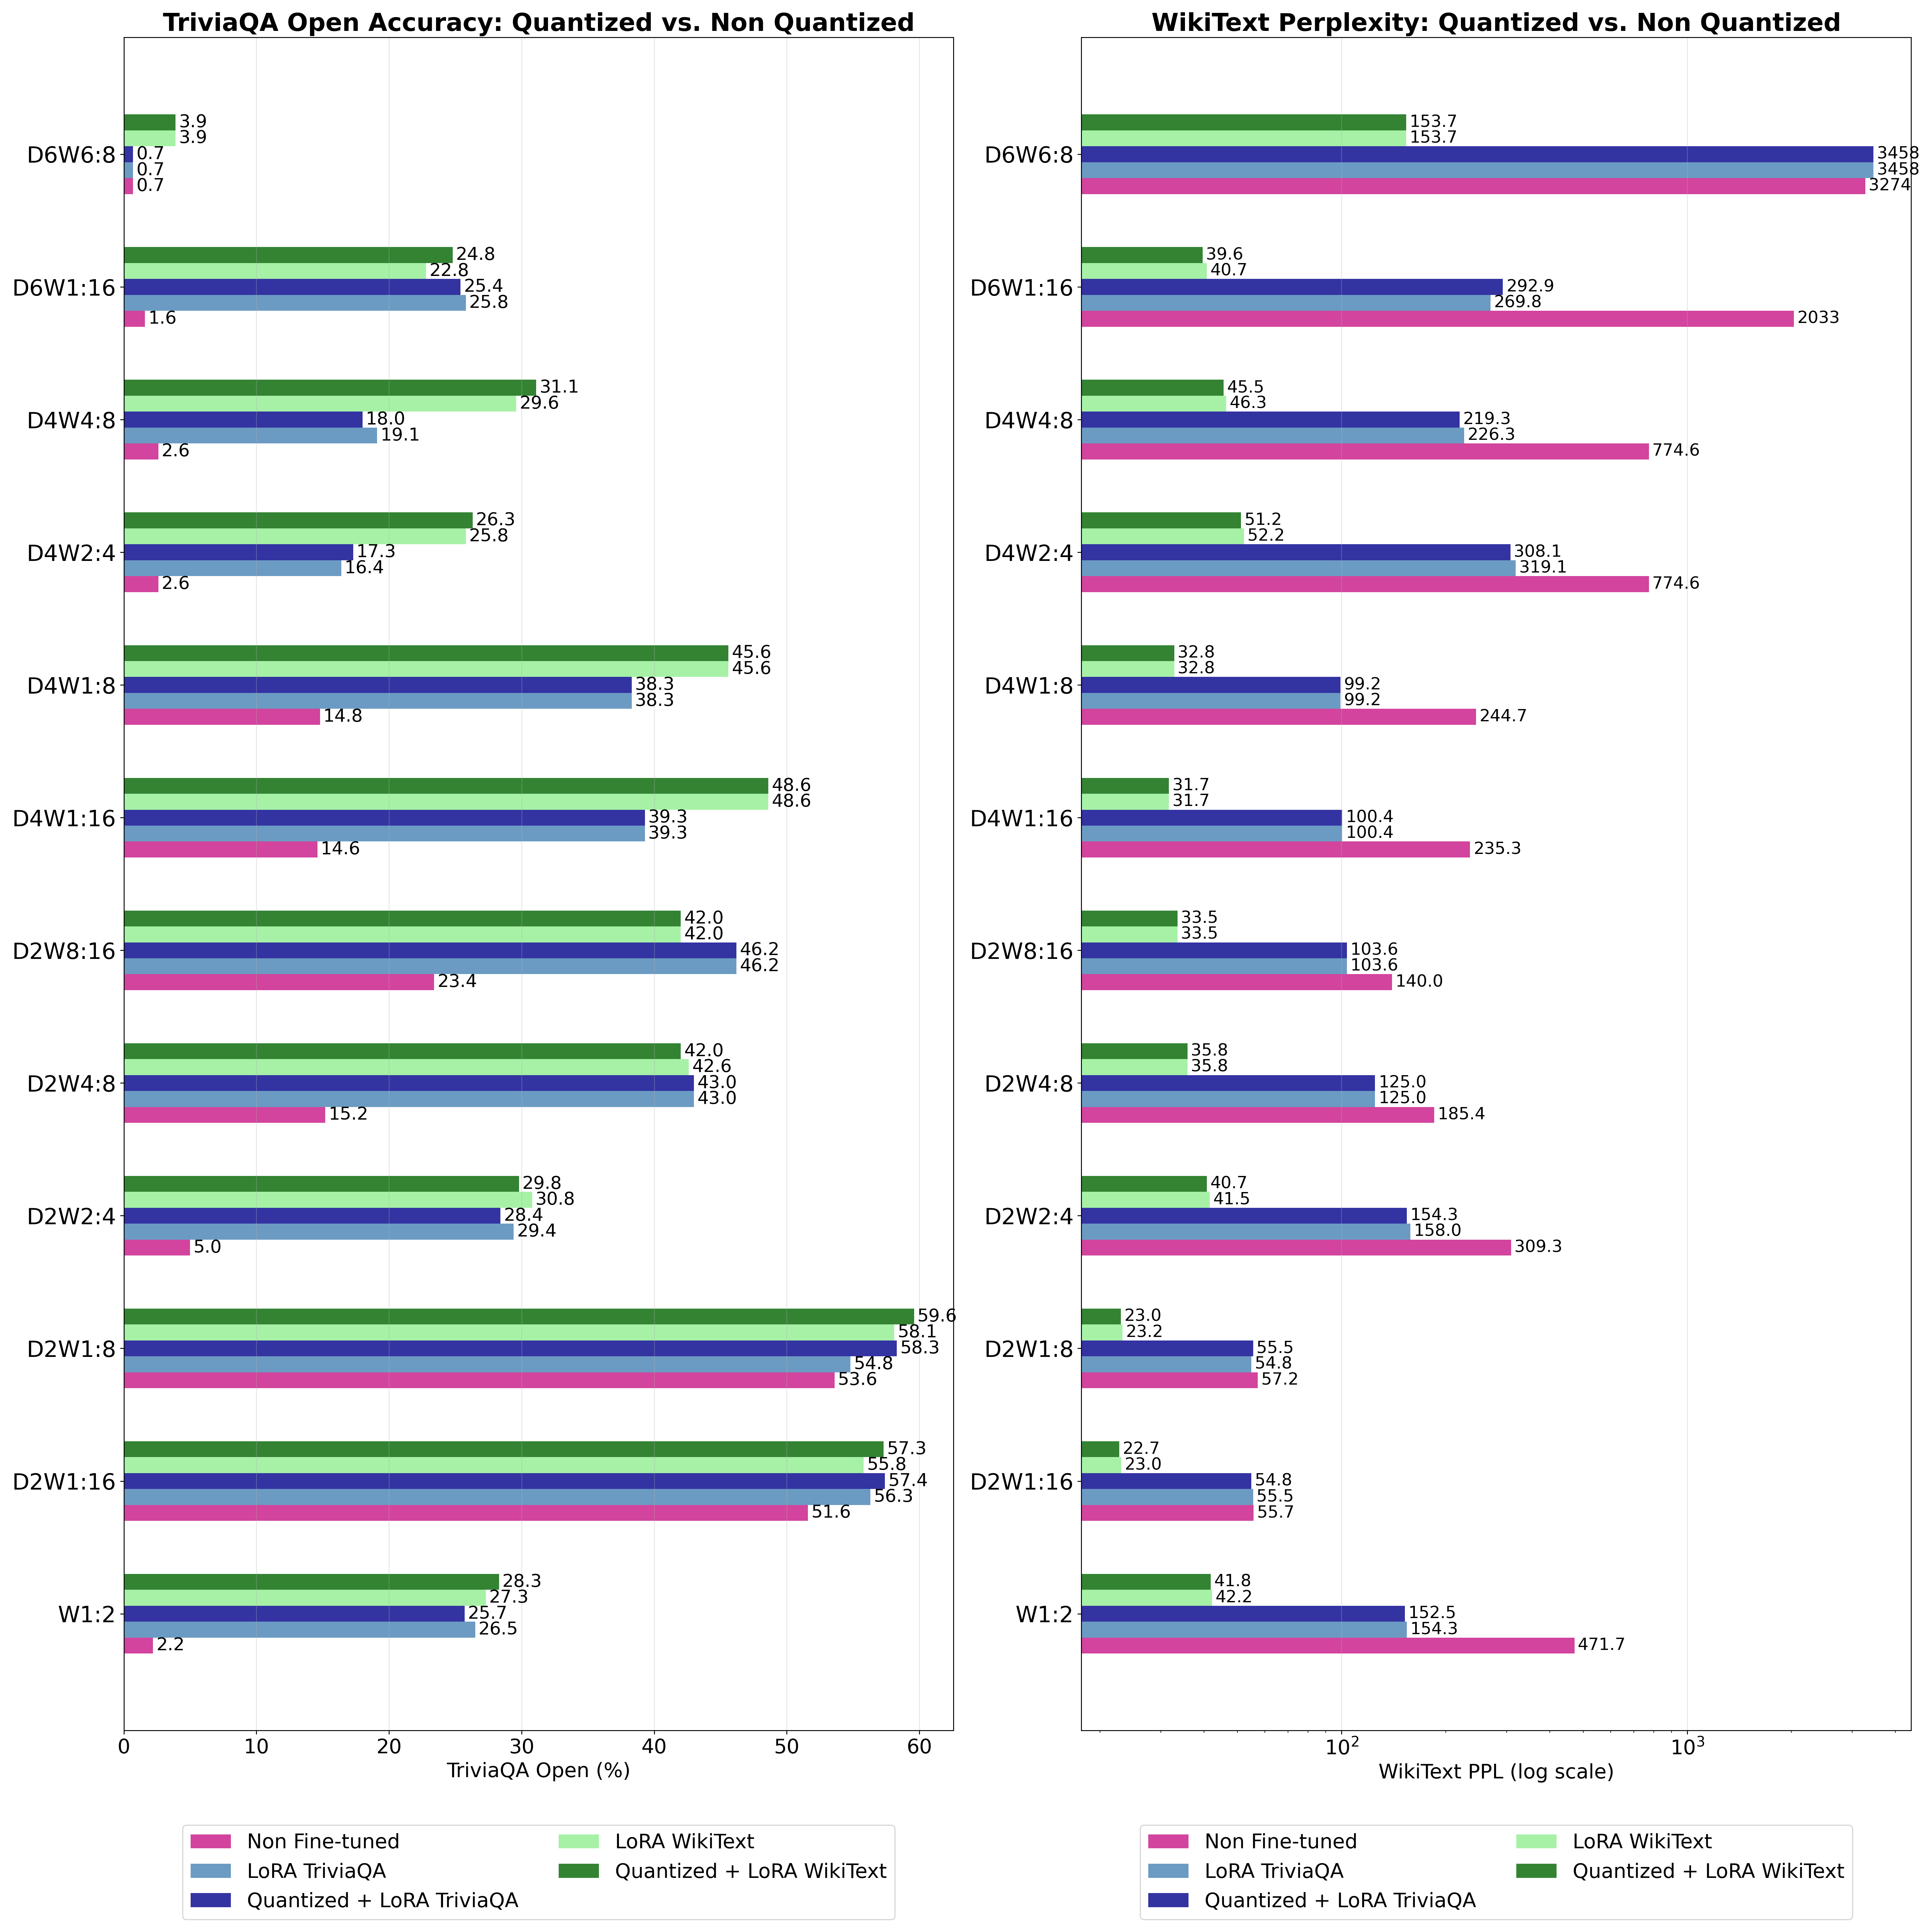
\includegraphics[width=\textwidth]{quant_graph.png}
    \caption[Comparison of Quantized and LoRA Models]{This figure shows a performance comparison of various pruned model configurations when LoRA fine-tuning and quantization are applied to them. Each configuration is evaluated under five conditions: the baseline pruned model, LoRA fine-tuning on WikiText, LoRA fine-tuning on TriviaQA, and both LoRA methods combined with quantization. Performance is measured using TriviaQA Open accuracy and WikiText perplexity metrics.}
    \label{fig:graph_quant}
\end{figure}

LoRA adaptation reveals significant effectiveness in recovering capabilities lost during pruning across all tested configurations. The Depth 2 variant exemplifies this recovery potential, with TriviaQA fine-tuning improving open-book performance from the pruned baseline of 53.0\% to 60.2\% and closed-book accuracy from 20.0\% to 27.8\%. The perplexity improvements are equally dramatic, with WikiText fine-tuning reducing perplexity from 55.24 to 21.34, bringing the compressed model's language modeling capabilities significantly closer to the original baseline. The Width 1:8 configuration demonstrates even more impressive recovery, maintaining 80.8\% TriviaQA Open performance while achieving remarkable perplexity reduction from 27.19 to 15.70 with WikiText fine-tuning. Figure \ref{fig:graph_quant} provides a visual comparison of a select set of configurations.

The recovery potential of LoRA becomes even more striking when dealing with heavily compressed models. For the aggressively pruned Depth 6 + Width 4:8 configuration, LoRA fine-tuning dramatically reduces perplexity from 554910 to 55.46, demonstrating that even severely degraded models can achieve substantial recovery. When quantization is applied to this setup, the model still maintains a perplexity of 58.80, which represents a reasonable score considering the extreme compression applied.

Interestingly, WikiText fine-tuning frequently outperforms TriviaQA fine-tuning across configurations, even when evaluated on TriviaQA benchmarks. For instance, the Width 1:2 variant with 4-bit quantization exhibits this pattern: WikiText LoRA achieves comparable TriviaQA open-book accuracy (27.3\% vs 26.5\%) while delivering dramatically better perplexity (42.19 vs 154.33) compared to TriviaQA LoRA. This pattern holds consistently across all optimization stages for this configuration, with WikiText variants achieving superior TriviaQA Open performance in the non-quantized (32.0\% vs 29.3\%) and EoRA-compensated (28.3\% vs 25.7\%) versions. This suggests that WikiText's broader linguistic diversity provides more effective adaptation for general language modeling capabilities, which translates to better overall results even on task-specific evaluations.


The addition of 4-bit quantization introduces a predictable trade-off between memory efficiency and quality. Across configurations, quantization typically causes 3-6 percentage point degradation on TriviaQA tasks, though this cost remains manageable given the substantial memory savings achieved through 4-bit representation. The Width 1:8 variant exemplifies this trade-off, dropping from 80.8\% to 74.8\% TriviaQA Open accuracy with quantization while maintaining excellent perplexity scores.

In contrast, EoRA compensation provides modest but consistent improvements over standard quantization. The technique typically recovers 1-2 percentage points of lost performance with minimal computational overhead. For the Depth 4 + Width 4:8 setting, EoRA improves accuracy from 29.6\% to 31.1\% TriviaQA Open while slightly reducing perplexity from 46.34 to 45.53. These gains, while incremental, show that EoRA provides only marginal quality improvements given its rather low computational overhead. A visualization of the effect of EoRA on the quantized models is illustrated in Figure \ref{fig:graph_eora}.

\begin{figure}[!htbp]
    \centering
    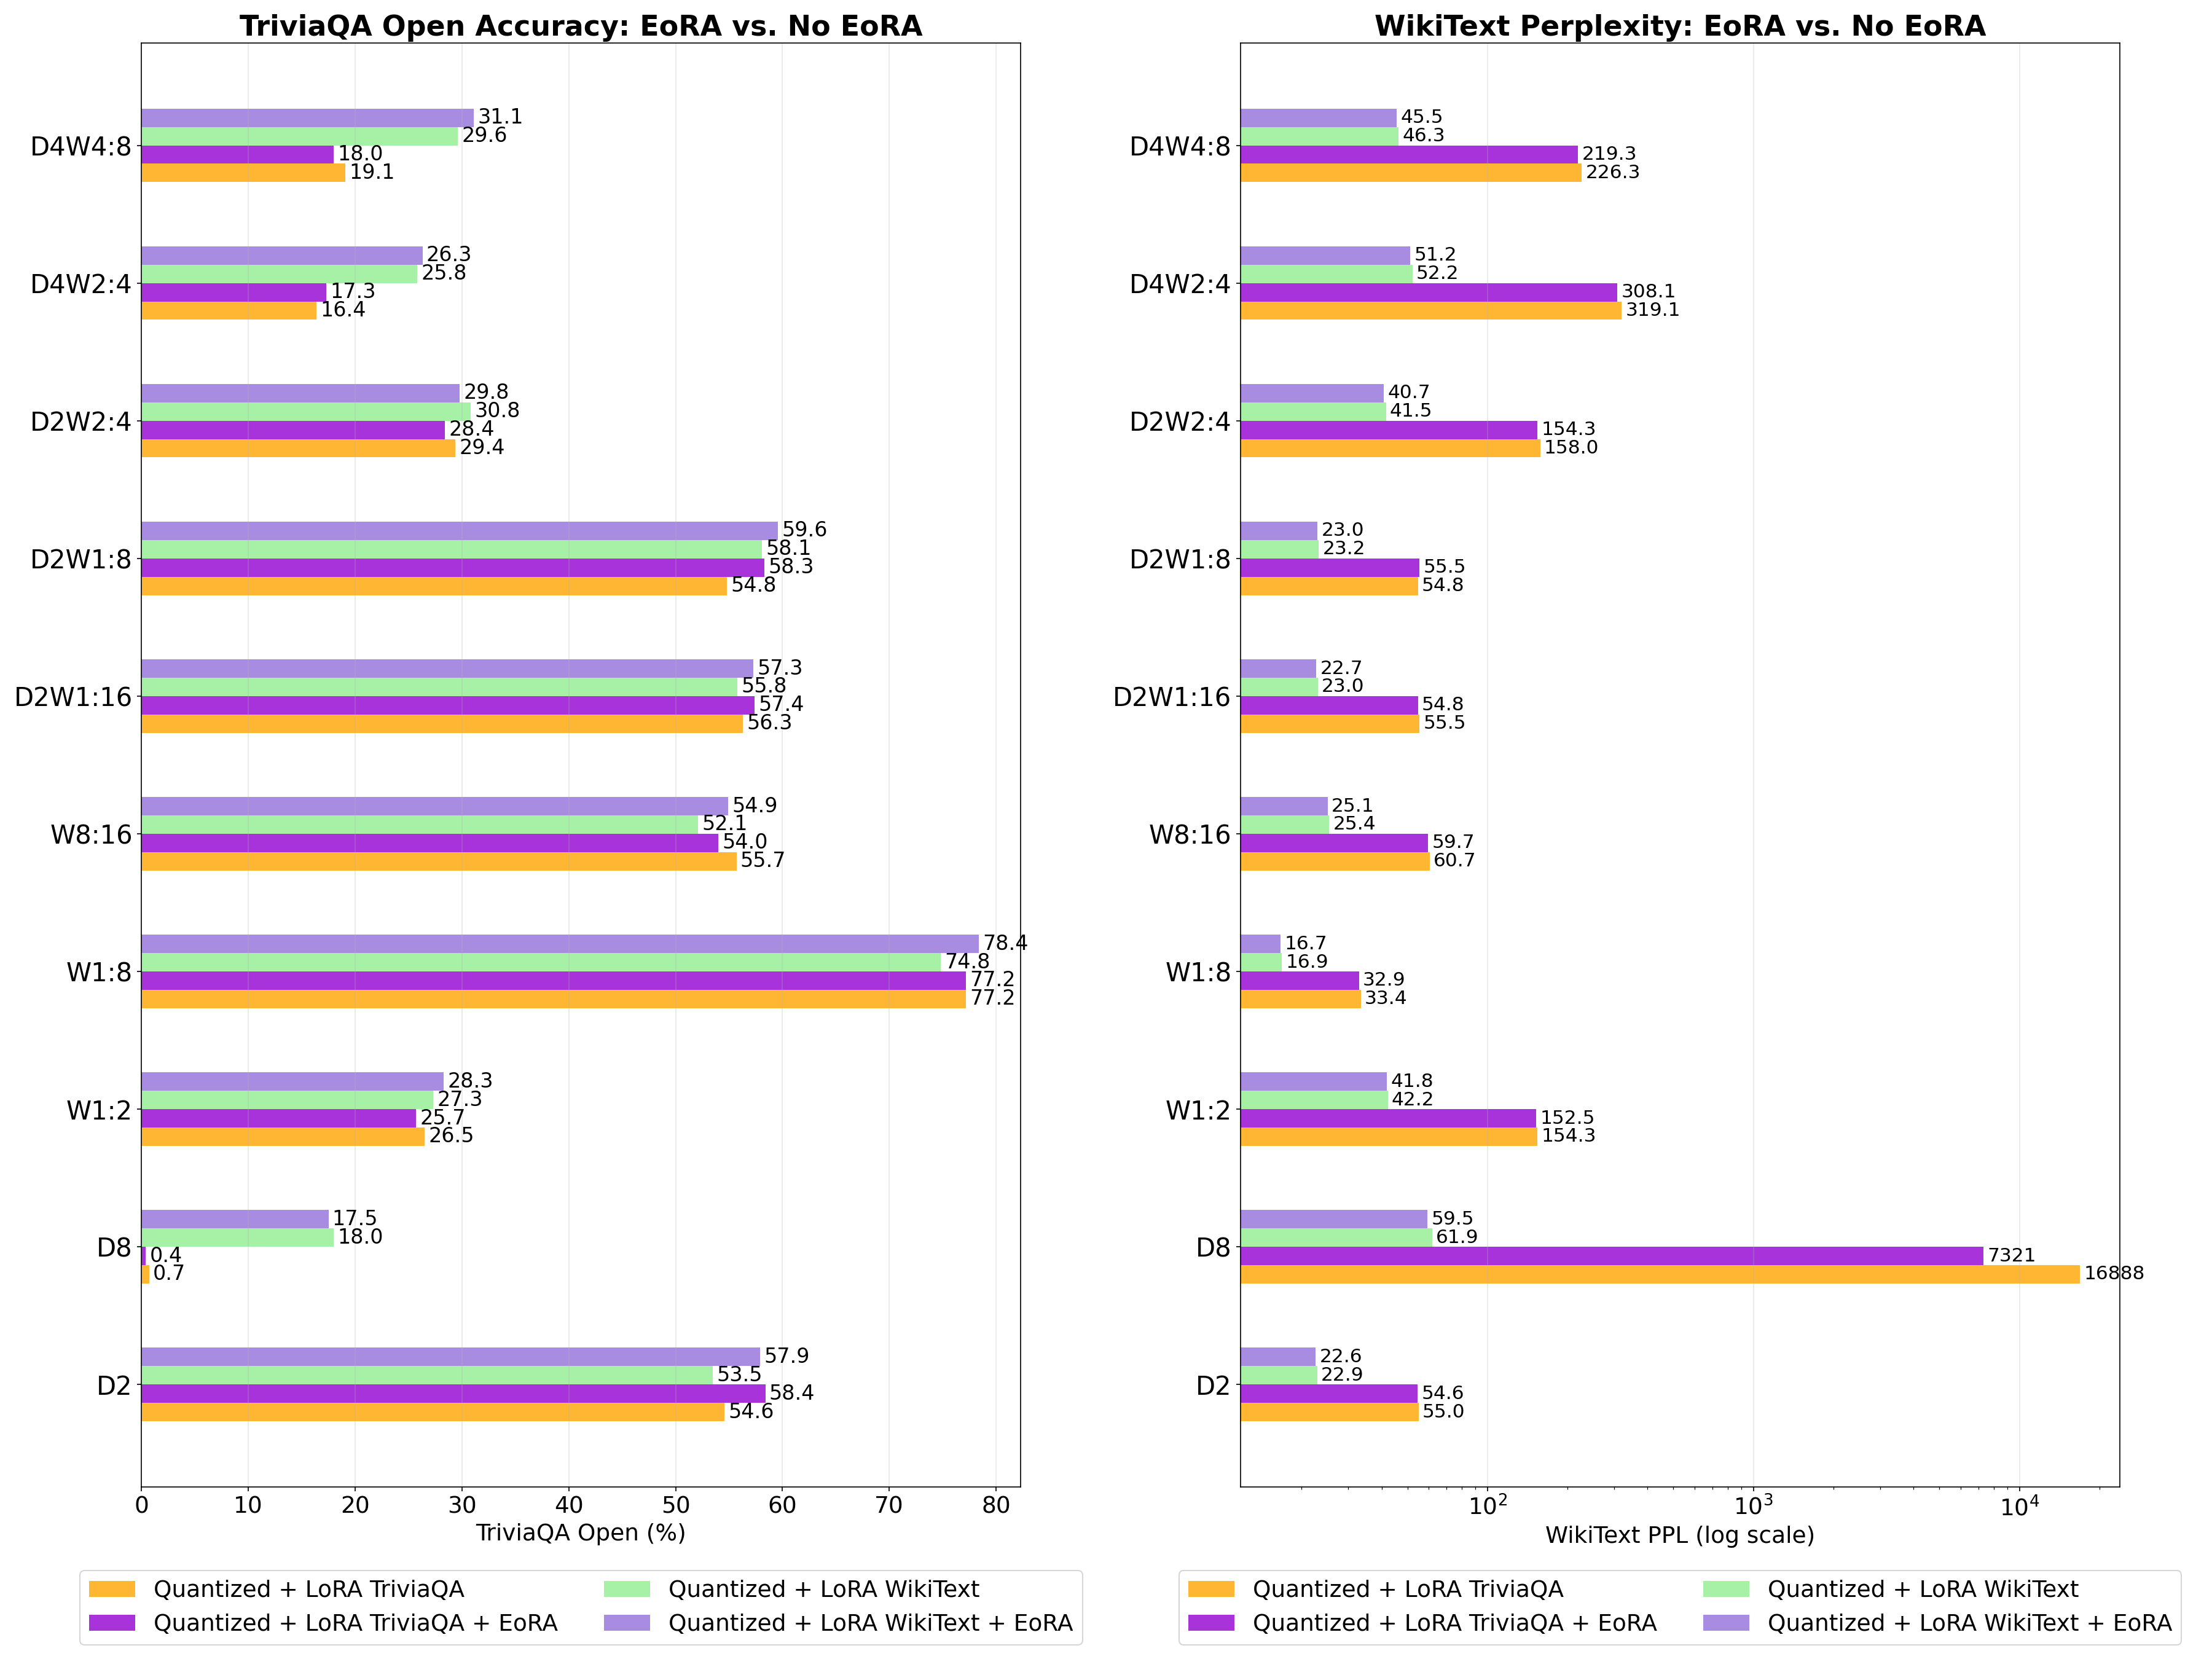
\includegraphics[width=\textwidth]{eora_graph.png}
    \caption[Comparison of Quantized and EoRA Models]{This figure shows the effect of EoRA on a subset of fine-tuned quantized model configurations. Each configuration is evaluated under four conditions: quantized LoRA fine-tuning on TriviaQA, quantized LoRA fine-tuning on WikiText, and both methods enhanced with EoRA performance recovery. Performance is measured using TriviaQA Open accuracy and WikiText perplexity metrics.}
    \label{fig:graph_eora}
\end{figure}

Nevertheless, even when recovery techniques are applied to the most compressed models, their performance degradation remains unsalvageable. The Depth 8 + Width 3:4 configuration demonstrates this limitation, where despite TriviaQA fine-tuning, the model yields essentially nil accuracy of only 0.3\% on both TriviaQA metrics with a perplexity of 7263.56, rendering it effectively unusable for practical applications.